\documentclass[conference]{IEEEtran}
\IEEEoverridecommandlockouts

\usepackage{cite}
\usepackage{amsmath,amssymb,amsfonts}
\usepackage{algorithmic}
\usepackage{graphicx}
\usepackage{textcomp}
\usepackage{xcolor}
\usepackage{booktabs}
\usepackage{url}
\usepackage{tikz}
\usetikzlibrary{arrows.meta,positioning,fit,backgrounds,calc}

% Colour used for the confusion-matrix heat map
\definecolor{cmblue}{RGB}{31,86,140}

\def\BibTeX{{\rm B\kern-.05em{\sc i\kern-.025em b}\kern-.08em
    T\kern-.1667em\lower.7ex\hbox{E}\kern-.125emX}}

\begin{document}

\title{AI-Powered Fish Disease Detection: Advancing Sustainable
Aquaculture through Mobile Deep Learning Solutions}

\maketitle

\begin{abstract}
Diagnosing fish disease at the pond edge is still, for the most part, a matter of visual judgment. While this can work reasonably well for experienced farmers, incorrect diagnosis can result in fish mortality and unnecessary treatment. AquaScan was developed to address this problem through an offline-first mobile and backend system that accepts a single fish photograph, processes it through a convolutional neural network trained on a seven-class freshwater fish disease taxonomy, and provides an actionable result rather than only a probability score. The system incorporates a fish-presence gate and an entropy-based rejection rule to prevent the closed-set classifier from forcing a disease prediction on photographs containing hands, walls, empty water, or other irrelevant content. A confidence-tiering mechanism further separates high-confidence predictions from uncertain results. In addition, AquaScan integrates a locally hosted retrieval-augmented generation assistant grounded in a curated aquaculture knowledge base, allowing users to ask follow-up questions and receive citation-supported answers without requiring a cloud language-model service. On a 700-image held-out test set, the production model achieved 81.3\% top-1 accuracy, 95.1\% top-3 accuracy, and a macro F1-score of 0.81. These results are reported as measured deployment-oriented performance and are not presented as a direct reproduction of the approximately 99.7\% benchmark reported by Tamut et al. \cite{b1}. The complete system combines deep learning, uncertainty handling, offline-first mobile application development, FastAPI services, FAISS retrieval, and local large language model inference to provide a practical decision-support tool for freshwater aquaculture.
\end{abstract}

\begin{IEEEkeywords}
fish disease classification, convolutional neural network, aquaculture, offline-first mobile systems, retrieval-augmented generation, uncertainty estimation, FastAPI, Flutter, local LLM
\end{IEEEkeywords}


% =========================================================
% I. INTRODUCTION
% =========================================================

\section{Introduction}

Freshwater aquaculture supports food security and rural livelihoods across South Asia, but disease outbreaks remain a major source of stock mortality and production loss. Early visual signs such as skin hemorrhage, fin rot, gill inflammation, fungal patches, or abnormal swimming may be misinterpreted by inexperienced operators, leading to delayed treatment or inappropriate interventions.

Image classification provides a potential method for shortening this diagnostic pathway. Tamut et al. developed a convolutional neural network (CNN) for seven-class South Asian freshwater fish disease classification and reported a benchmark accuracy of approximately 99.7\% under their experimental protocol \cite{b1}. This result demonstrates that the underlying visual classification problem is learnable. However, benchmark accuracy alone does not establish how a model behaves when exposed to uncontrolled pond-side photographs, non-fish images, ambiguous samples, or questions requiring contextual knowledge.

AquaScan extends the image-classification problem into an integrated decision-support application. The system combines a paper-aligned CNN \cite{b1} with an ImageNet-pretrained \cite{b26} MobileNetV2 \cite{b7} fish-presence gate, entropy-aware uncertainty filtering \cite{b24}, \cite{b25}, confidence-tiered prediction presentation, a FastAPI \cite{b15} inference backend, and a Flutter \cite{b14} mobile interface.

A second component is a locally deployed retrieval-augmented generation (RAG) assistant \cite{b4}. Rather than relying entirely on the internal knowledge of a general-purpose language model, AquaScan retrieves information from a curated aquaculture knowledge base and combines that context with the CNN prediction. The assistant can therefore explain a detected condition, answer follow-up questions, and provide grounded educational guidance while avoiding dependence on third-party cloud inference APIs.

The principal contributions of this work are:

\begin{itemize}
    \item A reproducible seven-class CNN implementation using a shared preprocessing contract across training, evaluation, and inference \cite{b1}.
    \item A production-oriented prediction pipeline containing a fish-presence gate, entropy-based rejection \cite{b24}, \cite{b25}, confidence tiers, and top-3 prediction reporting.
    \item A Flutter-based cross-platform mobile interface \cite{b14} connected to a FastAPI inference backend \cite{b15}.
    \item A local RAG architecture \cite{b4} using MiniLM embeddings \cite{b5}, FAISS retrieval \cite{b6}, and selectable GGUF language models served through \texttt{llama.cpp} \cite{b13}.
    \item An integrated approach that connects visual prediction, uncertainty handling, retrieval-grounded explanation, and conversational assistance.
\end{itemize}


% =========================================================
% II. RELATED WORK
% =========================================================

\section{Related Work}

Image-based fish disease recognition has increasingly benefited from deep learning because CNNs can learn visual patterns associated with lesions, discoloration, fungal growth, and other disease symptoms. Tamut et al. introduced a compact CNN for seven freshwater fish disease categories and provide the principal architectural basis for AquaScan \cite{b1}.

Transfer-learning architectures such as ResNet \cite{b8}, MobileNet \cite{b7}, and EfficientNet \cite{b9} have also been widely used when datasets are relatively small, and vision transformers \cite{b10} have more recently been applied to the same class of problems. These architectures provide useful baselines because they offer different trade-offs between representational capacity, inference cost, and deployment size. Their pretrained weights are typically derived from ImageNet \cite{b26}, which makes them practical starting points for domains with limited labeled data.

Modern training practice for such models depends heavily on regularization and normalization components: dropout \cite{b27} and batch normalization \cite{b28} stabilize the compact convolutional stack, label smoothing \cite{b29} discourages overconfident softmax outputs, and decoupled weight decay \cite{b11} improves generalization relative to the original Adam formulation \cite{b12}. Class-balanced losses \cite{b3} address the skewed class frequencies typical of curated disease datasets.

A separate line of work addresses what a closed-set classifier should do when the input falls outside its training distribution. Hendrycks and Gimpel established maximum softmax probability as a baseline for detecting misclassified and out-of-distribution inputs \cite{b25}, and Shannon entropy \cite{b24} provides a complementary measure of predictive uncertainty. Guo et al. showed that modern neural networks are frequently miscalibrated \cite{b23}, which motivates reporting expected calibration error alongside accuracy.

Retrieval-augmented generation has emerged as an approach for grounding language-model responses in external knowledge sources \cite{b4}. Rather than asking an LLM to generate an answer exclusively from parametric knowledge, a RAG pipeline retrieves relevant documents and provides those documents as context during generation.

AquaScan adapts this approach to aquaculture by combining disease metadata, aquaculture guidance, water-quality information, and prediction interpretation documents with locally hosted language models. FAISS \cite{b6} is used for vector similarity search, while sentence-transformers \cite{b5} provides semantic embeddings, and \texttt{llama.cpp} \cite{b13} performs quantized on-device generation.

The distinguishing characteristic of AquaScan is therefore not the CNN alone, but the integration of image classification, uncertainty filtering, mobile deployment, retrieval, and local language-model assistance into one system.


% =========================================================
% III. METHODOLOGY
% =========================================================

\section{Methodology}

\subsection{Research and Development Strategy}

AquaScan was developed as an integrated software research project across eleven milestones covering planning, literature review, dataset preparation, model development, backend development, frontend development, RAG knowledge-base construction, LLM integration, interface refinement, testing, performance optimization, and documentation.

The implementation separates model development from application orchestration. Training and evaluation are maintained within the backend training package, the FastAPI service \cite{b15} handles prediction and assistant APIs, and the Flutter application \cite{b14} manages capture, presentation, authentication, history, and conversation.

This separation allows the classifier or local language model to be replaced without requiring a redesign of the complete user interface.

\subsection{Dataset and Disease Taxonomy}

The classifier uses the public ``Freshwater Fish Disease Aquaculture in South Asia'' dataset containing 2,444 labeled images \cite{b2}. Seven disease classes are used for CNN training and evaluation. A synthetic eighth outcome, ``No Fish Detected,'' exists only at inference time and is produced when the fish-presence gate or uncertainty logic rejects an input.

\begin{table}[!t]
\caption{Disease Classes Used by AquaScan}
\centering
\scriptsize
\begin{tabular}{c l l}
\toprule
\textbf{Index} & \textbf{Disease Class} & \textbf{Type}\\
\midrule
0 & Bacterial Red Disease & Bacterial\\
1 & Bacterial Aeromoniasis & Bacterial\\
2 & Bacterial Gill Disease & Bacterial\\
3 & Fungal Saprolegniasis & Fungal\\
4 & Healthy Fish & Healthy\\
5 & Parasitic Disease & Parasitic\\
6 & Viral White Tail Disease & Viral\\
\bottomrule
\end{tabular}
\label{tab:diseaseclasses}
\end{table}

The test folder was kept isolated from training and model-selection decisions. Seven hundred images were used for final held-out evaluation. The project also performs a dataset audit for corrupted files, near-duplicates, and possible train-test leakage.

\subsection{CNN Model Development}

The paper-aligned CNN \cite{b1} accepts $150\times150\times3$ RGB input and normalizes pixel values to the range $[0,1]$ by division by 255.

The network contains three convolutional blocks with 128, 64, and 32 filters. The first block uses a $5\times5$ kernel while the remaining blocks use $3\times3$ kernels. Each convolutional block is followed by max pooling, batch normalization \cite{b28}, and dropout \cite{b27}. The resulting representation is flattened and passed through a 256-unit ReLU dense layer, followed by dropout and a seven-unit softmax output.

The architecture contains approximately 2.2 million parameters.

Training uses categorical cross-entropy with optional label smoothing of 0.05 \cite{b29}. AdamW \cite{b11} is used with a weight decay of $10^{-4}$, which decouples the regularization term from the adaptive step size of Adam \cite{b12}. Early stopping monitors validation loss with a patience of fifteen epochs. Class imbalance is addressed through inverse-frequency or effective-number class weighting \cite{b3}.

Data augmentation includes rotation, translation, horizontal flipping, zoom, and brightness variation.

A critical development lesson was preprocessing parity. Early versions used inconsistent resize and crop semantics between training and inference. The final system therefore implements a single preprocessing module responsible for image decoding, EXIF-aware rotation, RGB conversion, $150\times150$ LANCZOS resizing, normalization, and batch-dimension insertion.

\subsection{Baseline Model Comparison}

To strengthen the architectural justification, AquaScan defines a controlled baseline experiment in which alternative image-classification architectures are evaluated using the same dataset split, image preprocessing, augmentation policy, optimizer-selection procedure, and held-out test set.

The planned baseline set contains:

\begin{itemize}
    \item ResNet50 \cite{b8},
    \item EfficientNet-B0 \cite{b9},
    \item MobileNetV2 \cite{b7}, and
    \item a lightweight Vision Transformer (ViT) \cite{b10}.
\end{itemize}

The comparison should report top-1 accuracy, top-3 accuracy, macro precision, macro recall, macro F1, inference latency, and parameter count.

Importantly, only MobileNetV2 \cite{b7} was actually trained as a comparison model during the present development cycle, and it did not outperform the paper-aligned architecture on the project's split. Numerical results for ResNet50, EfficientNet-B0, and the lightweight ViT are not reported here because those experiments were not completed.

\begin{table}[!t]
\caption{Architecture Comparison Protocol}
\centering
\scriptsize
\begin{tabular}{l l l}
\toprule
\textbf{Architecture} & \textbf{Role} & \textbf{Status}\\
\midrule
Paper-aligned CNN \cite{b1} & Production model & Evaluated\\
MobileNetV2 \cite{b7} & Lightweight baseline & Evaluated\\
ResNet50 \cite{b8} & Strong CNN baseline & Future experiment\\
EfficientNet-B0 \cite{b9} & Efficient CNN baseline & Future experiment\\
Lightweight ViT \cite{b10} & Transformer baseline & Future experiment\\
\bottomrule
\end{tabular}
\label{tab:baselines}
\end{table}

This comparison protocol prevents architectural selection from being justified solely through inheritance from previous work and provides a direct path for future empirical validation.

\subsection{Inference Pipeline and Uncertainty Handling}

A closed-set classifier will always produce one of its known classes even when an input image is unrelated to the training domain \cite{b25}. AquaScan therefore implements a staged inference pipeline.

First, image-quality checks reject images smaller than 64 pixels on a side or images with clearly unsuitable aspect ratios. Second, an ImageNet-pretrained \cite{b26} MobileNetV2 model \cite{b7} functions as a fish-presence gate. The probabilities associated with seventeen fish-related ImageNet classes are summed, and an input is rejected when the combined probability is below 0.05.

If the fish gate is passed, the disease CNN generates its seven-class probability distribution. An entropy-based rejection rule \cite{b24} then rejects cases in which maximum class confidence \cite{b25} is below 0.20 and entropy exceeds 1.90.

The theoretical maximum entropy for a seven-class probability distribution is approximately:

\begin{equation}
H_{\max}=\log(7)\approx1.946.
\end{equation}

The final confidence tiers are:

\begin{itemize}
    \item \textbf{HIGH}: confidence $\geq 0.70$.
    \item \textbf{MEDIUM}: confidence between 0.45 and 0.70.
    \item \textbf{LOW}: confidence below 0.45 and explicitly presented as an indication rather than a diagnosis.
\end{itemize}

High-confidence predictions can display a direct recommended action, while medium-confidence results encourage the user to capture another photograph. Because softmax outputs are known to be poorly calibrated in modern networks \cite{b23}, these thresholds are treated as operating points selected for user-interface behavior rather than as calibrated posterior probabilities.

\begin{figure}[!t]
\centering
\includegraphics[width=0.34\columnwidth]{3app.jpg}
\caption{AquaScan prediction interface showing Bacterial Aeromoniasis with 93.0\% confidence, confidence tiering, recommended next action, and top predictions.}
\label{fig:prediction}
\end{figure}

Figure~\ref{fig:prediction} demonstrates how the application translates model output into a user-facing result. The interface does not display only a disease label; it also exposes confidence, alternative predictions, and a recommended next step.

\subsection{Fish-Presence Gate Evaluation}

The fish-presence gate is intended to reduce false-positive disease predictions on non-fish images. A dedicated evaluation should therefore distinguish between in-distribution fish photographs and out-of-distribution inputs, following the protocol conventions established for OOD detection benchmarks \cite{b25}.

The evaluation protocol should contain at least two groups:

\begin{enumerate}
    \item genuine fish images that should pass the gate, and
    \item non-fish or irrelevant images that should be rejected.
\end{enumerate}

The following metrics should be calculated:

\begin{equation}
Precision=\frac{TP}{TP+FP},
\end{equation}

\begin{equation}
Recall=\frac{TP}{TP+FN},
\end{equation}

and

\begin{equation}
FPR=\frac{FP}{FP+TN}.
\end{equation}

The final study should additionally report gate performance on out-of-distribution categories such as hands, empty water, walls, nets, equipment, and unrelated photographs.

The current AquaScan paper defines the gate and its threshold but does not contain a dedicated labeled gate-evaluation dataset. Consequently, precision, recall, false-positive rate, and OOD rejection percentages are not fabricated in this study and remain an explicit evaluation requirement.

\subsection{Classification Evaluation}

All primary classification metrics are calculated using the untouched 700-image test set with preprocessing identical to live inference.

The evaluation pipeline reports:

\begin{itemize}
    \item top-1 accuracy,
    \item top-3 accuracy,
    \item balanced accuracy,
    \item macro precision,
    \item macro recall,
    \item macro F1,
    \item log loss,
    \item Cohen's kappa \cite{b20},
    \item Matthews correlation coefficient \cite{b21},
    \item expected calibration error (ECE) \cite{b23},
    \item multiclass Brier score \cite{b22}, and
    \item a $7\times7$ confusion matrix.
\end{itemize}


% =========================================================
% IV. RESULTS AND DISCUSSION
% =========================================================

\section{Results and Discussion}

\subsection{Quantitative Classification Results}

The first trained checkpoint, Keras v1, achieved 69.4\% top-1 accuracy, 92.0\% top-3 accuracy, and a macro F1-score of 0.70.

The promoted Keras v2 model introduced AdamW \cite{b11}, L2 regularization, label smoothing \cite{b29}, stronger augmentation, and class weighting \cite{b3}. It achieved 81.3\% top-1 accuracy, 95.1\% top-3 accuracy, and a macro F1-score of 0.81.

The improvement in top-1 accuracy from v1 to v2 is:

\begin{equation}
81.3-69.4=11.9
\end{equation}

percentage points.

\begin{table}[!t]
\caption{Held-Out Test Set Classification Performance ($N=700$)}
\centering
\scriptsize
\begin{tabular}{l c c c}
\toprule
\textbf{Model} & \textbf{Top-1} & \textbf{Top-3} & \textbf{Macro F1}\\
\midrule
Legacy ONNX fallback & $\sim79.0\%$ & -- & --\\
Keras v1 & 69.4\% & 92.0\% & 0.70\\
Keras v2 & \textbf{81.3\%} & \textbf{95.1\%} & \textbf{0.81}\\
Tamut et al. \cite{b1} & $\sim99.7\%$ & -- & --\\
\bottomrule
\end{tabular}
\label{tab:performance}
\end{table}

The difference between AquaScan's 81.3\% held-out accuracy and the approximately 99.7\% result reported by Tamut et al. \cite{b1} must be interpreted carefully because the evaluation protocols are not identical. AquaScan reports the result obtained from its untouched test split rather than substituting validation performance for final test performance.

\subsection{Confidence Intervals}

Because the final held-out test set contains 700 observations, an approximate 95\% confidence interval can be reported for the measured accuracy using the Wilson binomial interval \cite{b17}.

For the promoted model with an observed accuracy of 81.3\%, the approximate 95\% confidence interval is:

\begin{equation}
CI_{95\%}\approx[78.2\%,84.0\%].
\end{equation}

For comparison, the corresponding intervals for the v1 top-1 accuracy and v2 top-3 accuracy are approximately 65.9--72.7\% and 93.2--96.5\%, respectively.

\begin{table}[!t]
\caption{Approximate 95\% Wilson Confidence Intervals \cite{b17}}
\centering
\scriptsize
\begin{tabular}{l c c}
\toprule
\textbf{Metric} & \textbf{Observed} & \textbf{95\% CI}\\
\midrule
Keras v1 top-1 & 69.4\% & 65.9--72.7\%\\
Keras v2 top-1 & 81.3\% & 78.2--84.0\%\\
Keras v2 top-3 & 95.1\% & 93.2--96.5\%\\
\bottomrule
\end{tabular}
\label{tab:confidence_intervals}
\end{table}

These intervals should be interpreted as uncertainty around the observed proportions. They do not establish that v2 is statistically superior to v1 because the paired per-image predictions required for an appropriate significance test \cite{b16}, \cite{b18} are not available in the paper.

\subsection{Statistical Significance}

A rigorous comparison between Keras v1 and v2 should use paired predictions on exactly the same test images. McNemar's test \cite{b16} is appropriate for comparing paired binary correctness outcomes and is the recommended procedure for comparing two classifiers evaluated on a single test set \cite{b18}, while bootstrap resampling \cite{b19} can provide confidence intervals for differences in accuracy and macro F1.

For future experiments comparing multiple architectures, statistical testing should be conducted using paired predictions from the same held-out samples. A significance threshold of $\alpha=0.05$ may be used after accounting for multiple comparisons where appropriate.

The current study does not claim a statistically significant improvement between v1 and v2 because the contingency counts required for McNemar's test \cite{b16} are not available in the final reported results. This limitation is preferable to reporting an unsupported significance claim.

\subsection{Confusion Matrix and Error Analysis}

The evaluation implementation exports a $7\times7$ confusion matrix containing the true and predicted disease classes. Reporting it is necessary because aggregate accuracy can conceal systematic class-level errors: a model with 81.3\% accuracy distributed evenly across classes and one that is near-perfect on five classes while failing on two are operationally very different systems.

The matrix uses the following class order, which is preserved in Fig.~\ref{fig:confusion} and Table~\ref{tab:perclass}:

\begin{center}
\scriptsize
Bacterial Red Disease,
Bacterial Aeromoniasis,
Bacterial Gill Disease,
Fungal Saprolegniasis,
Healthy Fish,
Parasitic Disease,
Viral White Tail Disease.
\end{center}

The class-level analysis identifies Parasitic Disease as the weakest v2 class by precision, at 0.69, confirming that this class is over-predicted. For comparison, the v1 model showed weak recall for Bacterial Red Disease at 0.55 and weak precision for Viral White Tail Disease at 0.48.

\begin{table}[!t]
\caption{Per-Class Performance of the Promoted Keras v2 Model}
\centering
\scriptsize
\begin{tabular}{l c c c c}
\toprule
\textbf{Class} & \textbf{Prec.} & \textbf{Rec.} & \textbf{F1} & \textbf{Support}\\
\midrule
Bacterial Red Disease      & 0.869 & 0.730 & 0.793 & 100\\
Bacterial Aeromoniasis     & 0.880 & 0.730 & 0.798 & 100\\
Bacterial Gill Disease     & 0.911 & 0.820 & 0.863 & 100\\
Fungal Saprolegniasis      & 0.824 & 0.840 & 0.832 & 100\\
Healthy Fish               & 0.798 & 0.950 & 0.868 & 100\\
Parasitic Disease          & 0.690 & 0.890 & 0.777 & 100\\
Viral White Tail Disease   & 0.785 & 0.730 & 0.756 & 100\\
\midrule
\textbf{Macro average}     & \textbf{0.822} & \textbf{0.813} & \textbf{0.812} & 700\\
\bottomrule
\end{tabular}
\label{tab:perclass}
\end{table}

Table~\ref{tab:perclass} shows that the test set is perfectly balanced at 100 images per class, so macro and weighted averages coincide. The precision--recall asymmetry is the informative signal: Parasitic Disease and Healthy Fish both have recall well above precision, meaning the model reaches for these two labels, while the three classes at 0.73 recall are the ones being drawn away from.

\begin{figure}[!t]
\centering
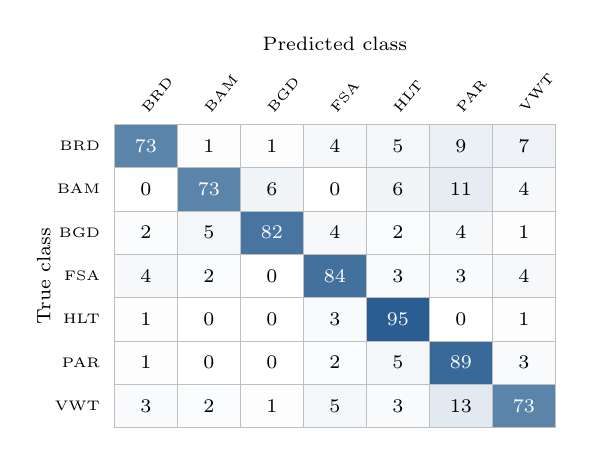
\begin{tikzpicture}[
  font=\scriptsize,
  cell/.style={draw=black!25, line width=0.2pt,
               minimum width=0.80cm, minimum height=0.55cm,
               inner sep=0pt, anchor=center}
]

% ---- column headers (predicted class) ----
\foreach \j/\lab in {0/BRD,1/BAM,2/BGD,3/FSA,4/HLT,5/PAR,6/VWT}
  \node[rotate=50, anchor=west, font=\tiny] at (\j*0.80-0.10, 0.36) {\lab};

% ---- row headers (true class) ----
\foreach \i/\lab in {0/BRD,1/BAM,2/BGD,3/FSA,4/HLT,5/PAR,6/VWT}
  \node[anchor=east, font=\tiny] at (-0.46, -\i*0.55) {\lab};

% ---- cells: row = true class, column = predicted class ----
\foreach \i/\j/\v in {%
  0/0/73, 0/1/1,  0/2/1,  0/3/4,  0/4/5,  0/5/9,  0/6/7,
  1/0/0,  1/1/73, 1/2/6,  1/3/0,  1/4/6,  1/5/11, 1/6/4,
  2/0/2,  2/1/5,  2/2/82, 2/3/4,  2/4/2,  2/5/4,  2/6/1,
  3/0/4,  3/1/2,  3/2/0,  3/3/84, 3/4/3,  3/5/3,  3/6/4,
  4/0/1,  4/1/0,  4/2/0,  4/3/3,  4/4/95, 4/5/0,  4/6/1,
  5/0/1,  5/1/0,  5/2/0,  5/3/2,  5/4/5,  5/5/89, 5/6/3,
  6/0/3,  6/1/2,  6/2/1,  6/3/5,  6/4/3,  6/5/13, 6/6/73}
  \node[cell, fill=cmblue!\v!white] at (\j*0.80, -\i*0.55)
        {\ifnum\v>50\relax\color{white}\fi\v};

% ---- axis titles ----
\node[font=\scriptsize] at (2.40, 1.30) {Predicted class};
\node[font=\scriptsize, rotate=90] at (-1.30, -1.65) {True class};

\end{tikzpicture}
\caption{Seven-class confusion matrix for the promoted Keras v2 model on the held-out test set ($N=700$, 100 images per class). Cell shading is proportional to the count; because every class has exactly 100 test images, each entry is simultaneously the row percentage. Class codes: BRD~=~Bacterial Red Disease, BAM~=~Bacterial Aeromoniasis, BGD~=~Bacterial Gill Disease, FSA~=~Fungal Saprolegniasis, HLT~=~Healthy Fish, PAR~=~Parasitic Disease, VWT~=~Viral White Tail Disease.}
\label{fig:confusion}
\end{figure}

Fig.~\ref{fig:confusion} shows the exported matrix. The diagonal sums to 569 of 700 images, which reproduces the 81.3\% top-1 accuracy reported in Table~\ref{tab:performance}. Two patterns dominate the residual error. First, the Parasitic Disease column absorbs 40 false positives, drawn from every class except Healthy Fish and most heavily from Viral White Tail Disease (13), Bacterial Aeromoniasis (11), and Bacterial Red Disease (9); this single column accounts for 30.5\% of the 131 total errors and explains the low 0.69 precision for that class despite its high 0.89 recall. Second, the Healthy Fish column attracts 24 false positives, drawn from all six other classes, meaning 4\% of diseased fish are declared healthy. Together these two columns account for 48.9\% of all errors. The three classes with the weakest recall, all at 0.73, are Bacterial Red Disease, Bacterial Aeromoniasis, and Viral White Tail Disease.

The asymmetry matters for deployment. Over-prediction of Parasitic Disease produces a recoverable error, since the recommended action is comparatively benign and the top-3 display will usually still contain the true class. False negatives routed into Healthy Fish are more consequential, because a healthy verdict terminates the diagnostic pathway rather than prompting further inspection. This suggests that class-conditional thresholds, rather than the single global confidence tiering described in Section~III, may be the more appropriate mechanism for the Healthy Fish class.

\subsection{Error Analysis}

The principal error sources identified during development were:

\begin{enumerate}
    \item preprocessing inconsistency between training and inference,
    \item class imbalance \cite{b3},
    \item visually similar disease symptoms,
    \item limited dataset size \cite{b2},
    \item controlled photographic conditions that may differ from pond-side images, and
    \item closed-set classification behavior on irrelevant inputs \cite{b25}.
\end{enumerate}

The preprocessing problem was particularly important. Early inference used semantics different from the training pipeline, producing low-confidence predictions on real camera photographs despite acceptable validation behavior. The final implementation uses one shared preprocessing module for training, evaluation, and inference.

The remaining class-level errors suggest that additional real-world images and grouped splitting by capture session would be valuable. Such a split would reduce the possibility that visually similar or near-duplicate images make the classification problem artificially easy.

\subsection{Dataset and External Validity}

The dataset \cite{b2} remains relatively small for a seven-class visual disease problem. Its photographic and geographic characteristics may not represent pond-side images containing variable lighting, water reflections, occlusion, camera-quality differences, fish orientation, or multiple fish.

The held-out test set therefore cannot establish performance across all species, farms, geographic regions, or camera devices. AquaScan should consequently be regarded as decision-support software rather than a veterinary diagnostic instrument.

\subsection{System Architecture}

AquaScan consists of three major layers:

\begin{enumerate}
    \item Flutter mobile client \cite{b14},
    \item FastAPI inference and assistant backend \cite{b15}, and
    \item local CNN, retrieval \cite{b6}, embedding \cite{b5}, and language-model \cite{b13} resources.
\end{enumerate}

The mobile client captures or selects an image and sends it to the backend. The backend performs image-quality checks, fish-presence screening, CNN classification, uncertainty filtering, and confidence-tier generation. The resulting prediction can then be attached to the local assistant session.

\begin{figure*}[!t]
\centering
\resizebox{\textwidth}{!}{%
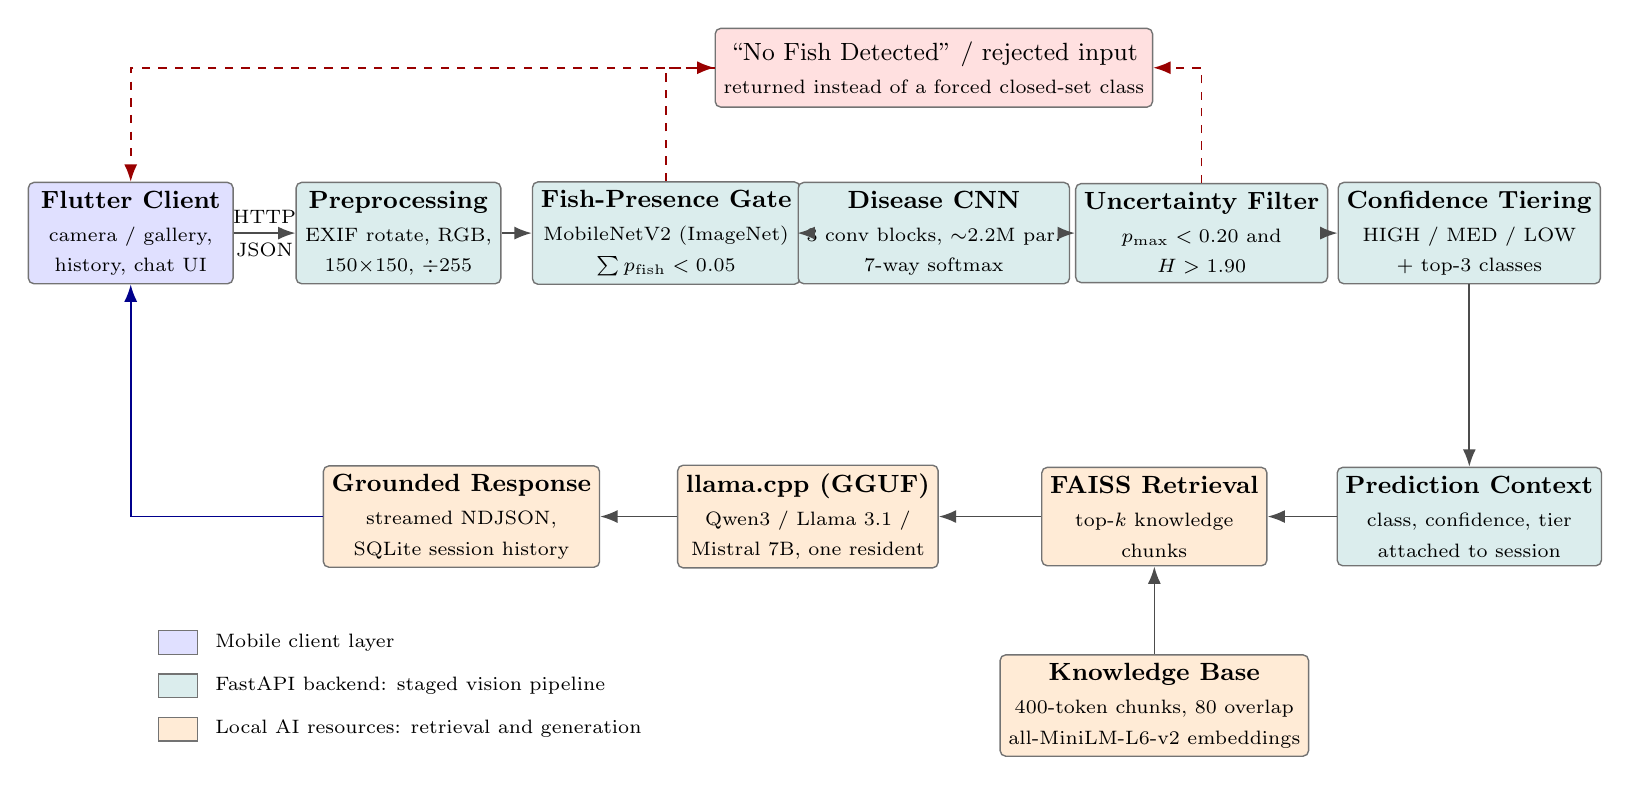
\begin{tikzpicture}[
  font=\small,
  box/.style={rounded corners=2pt, draw=black!55, line width=0.5pt,
              minimum width=2.6cm, minimum height=1.25cm,
              align=center, inner sep=3pt},
  client/.style={box, fill=blue!12},
  svc/.style={box, fill=teal!14},
  ai/.style={box, fill=orange!16},
  rej/.style={box, fill=red!12, minimum width=5.0cm, minimum height=1.0cm},
  flow/.style={-{Latex[length=2.2mm]}, line width=0.6pt, draw=black!70},
  rflow/.style={-{Latex[length=2.2mm]}, line width=0.6pt,
                draw=red!60!black, dashed},
  back/.style={-{Latex[length=2.2mm]}, line width=0.6pt,
               draw=blue!55!black}
]

% ================= rejection branch (top) =================
\node[rej] (reject) at (10.2,2.1)
  {``No Fish Detected'' / rejected input\\[1pt]
   {\scriptsize returned instead of a forced closed-set class}};

% ================= vision pipeline (middle row) =================
\node[client] (client) at (0,0)
  {\textbf{Flutter Client}\\[1pt]
   {\scriptsize camera / gallery,}\\
   {\scriptsize history, chat UI}};
\node[svc] (prep) at (3.4,0)
  {\textbf{Preprocessing}\\[1pt]
   {\scriptsize EXIF rotate, RGB,}\\
   {\scriptsize $150{\times}150$, $\div 255$}};
\node[svc] (gate) at (6.8,0)
  {\textbf{Fish-Presence Gate}\\[1pt]
   {\scriptsize MobileNetV2 (ImageNet)}\\
   {\scriptsize $\sum p_{\mathrm{fish}} < 0.05$}};
\node[svc] (cnn) at (10.2,0)
  {\textbf{Disease CNN}\\[1pt]
   {\scriptsize 3 conv blocks, $\sim$2.2M par.}\\
   {\scriptsize 7-way softmax}};
\node[svc] (unc) at (13.6,0)
  {\textbf{Uncertainty Filter}\\[1pt]
   {\scriptsize $p_{\max} < 0.20$ and}\\
   {\scriptsize $H > 1.90$}};
\node[svc] (tier) at (17.0,0)
  {\textbf{Confidence Tiering}\\[1pt]
   {\scriptsize HIGH / MED / LOW}\\
   {\scriptsize + top-3 classes}};

\draw[flow] (client) -- node[above,font=\scriptsize]{HTTP}
                        node[below,font=\scriptsize]{JSON} (prep);
\draw[flow] (prep) -- (gate);
\draw[flow] (gate) -- (cnn);
\draw[flow] (cnn)  -- (unc);
\draw[flow] (unc)  -- (tier);

\draw[rflow] (gate) |- (reject);
\draw[rflow] (unc)  |- (reject);
\draw[rflow] (reject) -| (client);

% ================= RAG assistant (bottom row) =================
\node[svc] (ctx) at (17.0,-3.6)
  {\textbf{Prediction Context}\\[1pt]
   {\scriptsize class, confidence, tier}\\
   {\scriptsize attached to session}};
\node[ai] (faiss) at (13.0,-3.6)
  {\textbf{FAISS Retrieval}\\[1pt]
   {\scriptsize top-$k$ knowledge}\\
   {\scriptsize chunks}};
\node[ai] (llm) at (8.6,-3.6)
  {\textbf{llama.cpp (GGUF)}\\[1pt]
   {\scriptsize Qwen3 / Llama 3.1 /}\\
   {\scriptsize Mistral 7B, one resident}};
\node[ai] (resp) at (4.2,-3.6)
  {\textbf{Grounded Response}\\[1pt]
   {\scriptsize streamed NDJSON,}\\
   {\scriptsize SQLite session history}};
\node[ai] (kb) at (13.0,-6.0)
  {\textbf{Knowledge Base}\\[1pt]
   {\scriptsize 400-token chunks, 80 overlap}\\
   {\scriptsize all-MiniLM-L6-v2 embeddings}};

\draw[flow] (tier)  -- (ctx);
\draw[flow] (ctx)   -- (faiss);
\draw[flow] (faiss) -- (llm);
\draw[flow] (llm)   -- (resp);
\draw[flow] (kb)    -- (faiss);
\draw[back] (resp)  -| (client);

% ================= legend =================
% Placed in the empty lower-left region so that it does not
% collide with the two return arrows routed along x = 0.
\begin{scope}[shift={(0.6,-5.2)}, font=\scriptsize,
              sw/.style={draw=black!55, line width=0.4pt,
                         minimum width=0.5cm, minimum height=0.3cm,
                         inner sep=0pt}]
  \node[sw, fill=blue!12]   at (0,0)     {};
  \node[anchor=west]        at (0.35,0)  {Mobile client layer};
  \node[sw, fill=teal!14]   at (0,-0.55) {};
  \node[anchor=west]        at (0.35,-0.55) {FastAPI backend: staged vision pipeline};
  \node[sw, fill=orange!16] at (0,-1.10) {};
  \node[anchor=west]        at (0.35,-1.10) {Local AI resources: retrieval and generation};
\end{scope}

\end{tikzpicture}%
}
\caption{End-to-end AquaScan system architecture. Solid arrows show the nominal path: the Flutter client posts an image, the backend preprocesses it, screens it through the fish-presence gate, classifies it with the disease CNN, filters uncertain outputs, and returns a confidence-tiered result. Dashed red arrows show the two rejection paths that return ``No Fish Detected'' rather than forcing a closed-set class. The prediction is then attached as context to the local RAG assistant, whose grounded response returns to the client (blue arrow). Only one GGUF language model is resident in memory at a time.}
\label{fig:architecture}
\end{figure*}

Figure~\ref{fig:architecture} illustrates the separation between visual inference and language generation. The CNN produces a structured prediction, while the RAG assistant \cite{b4} provides contextual explanation using retrieved aquaculture information. The two dashed paths are the architectural expression of the uncertainty argument in Section~III: rejection is a first-class outcome of the pipeline rather than an error condition, and it can be triggered either before classification, by the fish-presence gate, or after it, by the entropy filter.

\subsection{Mobile Client and User Experience}

The mobile client is implemented using Flutter \cite{b14} and Material 3. It provides camera and gallery capture, disease-library access, scan history, authentication, theme control, and backend health monitoring.

\begin{figure}[!t]
\centering
\includegraphics[width=0.30\columnwidth]{1app.jpg}
\caption{AquaScan home interface showing AI status, seven-class CNN configuration, camera and gallery input, detectable conditions, and scan workflow.}
\label{fig:home}
\end{figure}

The home interface shown in Fig.~\ref{fig:home} provides the primary entry point into the system. Users can verify that the AI backend is available, initiate a scan, review detectable conditions, and navigate to the application library and history.

\begin{figure}[!t]
\centering
\includegraphics[width=0.30\columnwidth]{2app.jpg}
\caption{AquaScan scan interface showing camera and gallery input, detectable disease conditions, image-analysis stages, and image-capture guidance.}
\label{fig:scan}
\end{figure}

The scan interface in Fig.~\ref{fig:scan} presents the capture workflow and provides guidance for selecting a suitable photograph. This interface is designed to reduce avoidable input-quality problems before inference.

\subsection{Backend and Deployment}

The backend is implemented using FastAPI \cite{b15} and Uvicorn. The service exposes endpoints for health monitoring, model information, disease metadata, prediction, assistant status, RAG chat, streaming responses, prediction-context attachment, and knowledge-base reindexing.

The system supports Keras and ONNX model artifacts and uses local resources for embedding \cite{b5}, retrieval \cite{b6}, and LLM generation \cite{b13}. Only one GGUF language model is loaded into memory at a time to conserve system resources.

The current deployment is offline-first rather than strictly phone-only. After model and dependency installation, the backend can operate from local resources, while the Flutter client communicates through loopback or LAN addressing.

This architecture trades cloud scalability for greater privacy, connectivity independence, and control over the knowledge base.

\subsection{Engineering Challenges}

The development process revealed several cross-stack challenges. These included preprocessing inconsistencies, Android MIME-type handling, physical-device network addressing, Python and compiled dependency compatibility, and memory consumption when CNN inference, MiniLM embeddings \cite{b5}, FAISS retrieval \cite{b6}, and an 8B language model \cite{b13} were used on the same machine.

Physical Android devices cannot directly use emulator-specific loopback addressing, and local HTTP communication may require explicit configuration. These issues were mitigated through configurable backend addresses and pinned environments.

The system also uses lazy loading and configurable GPU offloading for local LLM inference to reduce memory pressure.


% =========================================================
% V. LLM INTEGRATION
% =========================================================

\section{LLM Integration}

\subsection{Local Aquaculture Assistant}

The classification result alone does not answer all practical questions a farmer may have. AquaScan therefore integrates a locally hosted language-model assistant that can explain predictions and answer follow-up aquaculture questions.

The assistant uses a curated knowledge base containing information related to water quality, biosecurity, species and feeding, common conditions, and interpretation of model predictions.

The CNN prediction can automatically be attached to the assistant session. This allows a user to ask contextual questions such as what a detected disease means, what symptoms are associated with the condition, or what immediate husbandry actions should be considered.

\begin{figure}[!t]
\centering
\includegraphics[width=0.30\columnwidth]{4app.jpg}
\caption{AquaScan local aquaculture assistant using Qwen3 to provide contextual information about the detected disease and observed symptoms.}
\label{fig:assistant}
\end{figure}

Figure~\ref{fig:assistant} demonstrates the integration between CNN output and conversational assistance. In the demonstrated interaction, the assistant receives the Bacterial Aeromoniasis prediction and uses it as context when answering the user's question.

\subsection{RAG Pipeline}

The RAG pipeline \cite{b4} uses domain documents that are divided into approximately 400-token chunks with an overlap of 80 tokens. Each chunk is embedded using \texttt{all-MiniLM-L6-v2} \cite{b5} and stored in a FAISS vector index \cite{b6}.

At query time, the system retrieves the most relevant knowledge chunks and combines them with the user's question and, when available, the current CNN prediction.

The resulting context is supplied to a locally hosted GGUF language model through \texttt{llama.cpp} \cite{b13}. Supported models include Llama 3.1, Mistral 7B, and Qwen3.

\subsection{RAG Evaluation Framework}

A formal RAG evaluation is necessary before claiming that the assistant improves response quality or reduces hallucination \cite{b4}.

The proposed benchmark should contain representative aquaculture questions from at least five categories:

\begin{enumerate}
    \item disease identification and symptom interpretation,
    \item water-quality and environmental questions,
    \item prevention and biosecurity,
    \item prediction-linked follow-up questions, and
    \item safety-sensitive treatment questions.
\end{enumerate}

Each question should have a reference answer and an expert-reviewed set of relevant source documents.

The following metrics should be reported.

\textbf{Retrieval accuracy:} whether the relevant knowledge chunk is retrieved within the top-$k$ results.

\begin{equation}
Recall@k =
\frac{\text{relevant queries retrieved in top-}k}
{\text{total relevant queries}}.
\end{equation}

\textbf{Grounding quality:} whether claims in the generated response are supported by retrieved source material.

\textbf{Citation correctness:} whether each citation actually supports the claim for which it is presented.

\textbf{Hallucination frequency:} proportion of generated factual claims that cannot be supported by the retrieved context.

\begin{equation}
HF =
\frac{\text{unsupported factual claims}}
{\text{total factual claims}}.
\end{equation}

\textbf{Response relevance:} whether the generated response directly addresses the user's question.

\textbf{Conciseness:} whether the response provides sufficient information without unnecessary repetition.

The same benchmark should be run across Llama 3.1, Mistral 7B, and Qwen3 using identical prompts and retrieved contexts. Human expert review should be combined with automated metrics.

The present AquaScan study does not report numerical RAG accuracy, grounding, citation correctness, or hallucination-frequency results because a formal aquaculture-specific benchmark has not yet been completed.

\subsection{LLM Safety and Grounding}

The assistant is explicitly instructed to treat the CNN confidence value as a probability estimate rather than a definitive diagnosis. This instruction is motivated by the known miscalibration of softmax confidence in deep networks \cite{b23}. Low-confidence and ``No Fish Detected'' results should not be converted into confident disease claims.

The assistant also avoids prescribing specific antibiotic dosages and encourages professional confirmation for major treatment decisions.

The system is therefore intended as educational and decision-support software rather than a replacement for aquatic veterinary diagnosis.

\subsection{Local Model Serving}

LLM inference is performed through quantized GGUF models using \texttt{llama.cpp} \cite{b13}. Token streaming is implemented using newline-delimited JSON so that the Flutter client \cite{b14} can display responses incrementally.

Chat history is maintained per session using SQLite. A persistent session identifier allows conversations to continue after application restart.


% =========================================================
% VI. FUTURE WORK
% =========================================================

\section{Future Work}

The present study establishes a working end-to-end system and an honest performance baseline. The work that follows is therefore organized around closing the specific evidentiary gaps identified in Section~IV and Section~V, rather than around adding new features. Each subsection below states the objective, the experimental design required to reach it, and the criterion by which the result should be judged.

\subsection{Model Development and Architectural Validation}

The first priority is a controlled comparison against stronger image-classification architectures. ResNet50 \cite{b8}, EfficientNet-B0 \cite{b9}, MobileNetV2 \cite{b7}, and a lightweight Vision Transformer \cite{b10} should be trained using identical data splits, preprocessing, augmentation policy, and evaluation protocol so that any observed difference is attributable to architecture rather than to training configuration.

Each architecture should be evaluated using top-1 accuracy, top-3 accuracy, macro precision, macro recall, macro F1, expected calibration error \cite{b23}, Brier score \cite{b22}, parameter count, and inference latency on both workstation and mobile hardware. The paper-aligned CNN \cite{b1} should be retained as the production model only if it is not significantly outperformed once accuracy is considered jointly with latency and model size. This makes the architectural choice falsifiable rather than inherited.

The dataset \cite{b2} should also be expanded with real pond-side photographs collected under variable lighting, turbidity, and camera quality. Grouped train-test splitting by capture session should be used to reduce the risk that near-duplicate frames inflate apparent performance. A target of several hundred additional field images per class would materially change the external-validity argument in Section~IV.

Active learning \cite{b32} could allow field-submitted misclassifications to become reviewed training examples, creating a feedback loop in which deployment improves the model rather than merely consuming it. Explainability methods such as Grad-CAM \cite{b30} should also be introduced so that a prediction can be accompanied by the image region that drove it. This matters for user trust: a heat map concentrated on a lesion is credible, whereas one concentrated on background water indicates that the model has learned a spurious correlate.

\subsection{Fish-Gate and Out-of-Distribution Evaluation}

A dedicated fish-gate dataset should be constructed containing both valid fish images and representative non-fish images drawn from the categories actually encountered in the field: hands, nets, buckets, pond surfaces, walls, feed bags, equipment, and unrelated photographs.

The evaluation should report precision, recall, specificity, false-positive rate, false-negative rate, and per-category rejection performance, following established out-of-distribution detection practice \cite{b25}.

Threshold sensitivity should also be evaluated around the current 0.05 fish-presence threshold. A receiver operating characteristic curve over the summed fish-class probability would show whether the selected operating point provides an appropriate trade-off between rejecting irrelevant inputs and incorrectly rejecting valid fish photographs. The asymmetry matters in deployment: incorrectly rejecting a genuine fish photograph is an inconvenience, whereas confidently returning a disease label for a photograph of a hand undermines trust in the entire system.

A complementary direction is to replace the summed-ImageNet-probability heuristic with a small purpose-trained binary fish detector, and to compare the two under the same protocol.

\subsection{Confusion Matrix and Systematic Error Analysis}

The confusion matrix in Fig.~\ref{fig:confusion} establishes \emph{where} the residual error concentrates but not \emph{why}. The natural continuation is a qualitative audit of the specific confusion pairs it exposes.

The 40 false positives in the Parasitic Disease column and the 24 in the Healthy Fish column together account for approximately half of all errors, so a review of those two columns alone would cover most of the remaining performance gap. Representative misclassified images should be examined manually to determine whether the errors arise from genuine visual similarity between conditions, image quality, occlusion, or insufficient training examples for the affected classes.

Pairing this qualitative review with Grad-CAM visualizations \cite{b30} would distinguish true visual ambiguity from model attention failures. If the attention maps for images misrouted into Parasitic Disease concentrate on lesion regions, the problem is genuine inter-class similarity and calls for more data or a finer-grained taxonomy; if they concentrate on background or fin edges, the model has learned a spurious correlate and the remedy is a change of loss or architecture. Distinguishing these two cases is the single most informative next experiment, because the current aggregate metrics cannot separate them.

\subsection{Formal LLM and Retrieval Evaluation}

The RAG assistant \cite{b4} should be evaluated using a fixed aquaculture benchmark containing disease, husbandry, water-quality, prevention, prediction-linked, ambiguous, and safety-sensitive questions, with reference answers and expert-annotated source passages.

Llama 3.1, Mistral 7B, and Qwen3 should be compared under identical retrieval conditions, prompts, and decoding parameters, so that observed differences reflect the generator rather than the retrieval stage.

The evaluation should report retrieval Recall@1 and Recall@4 \cite{b6}, response relevance, groundedness, citation correctness, unsupported-claim rate, hallucination frequency, response length, and end-to-end latency. An ablation in which retrieval is disabled should also be included, since the central claim of the RAG design is that retrieval reduces unsupported claims relative to the parametric-only baseline; without that ablation the claim remains untested.

Expert review by aquaculture or fisheries professionals should be included for treatment and disease-management questions, with particular attention to whether the assistant appropriately declines to give dosage-level guidance and appropriately escalates low-confidence predictions.

\subsection{Statistical Evaluation Protocol}

Future model comparisons should use paired predictions on the same held-out test samples, stored per image so that contingency tables can be constructed after the fact.

For two classifiers, McNemar's test \cite{b16} should be used to evaluate differences in paired correctness, as recommended for the single-test-set comparison setting \cite{b18}. Bootstrap resampling \cite{b19} should be used to estimate confidence intervals for accuracy, macro F1, and the difference between models, since macro F1 has no convenient closed-form interval.

For more than two architectures, multiple-comparison corrections should be applied to avoid inflating the family-wise error rate.

The significance level should be defined before testing, for example:

\begin{equation}
\alpha=0.05.
\end{equation}

This procedure will prevent model-selection conclusions from being based solely on small differences in aggregate accuracy, and will allow the improvement from v1 to v2 reported in Section~IV to be restated as a tested claim rather than an observed difference.

\subsection{Calibration and Threshold Selection}

The confidence tiers described in Section~III were selected as interface operating points rather than derived from calibrated probabilities. Because deep networks are frequently overconfident \cite{b23}, a calibration study should measure expected calibration error and reliability diagrams for the promoted model, and evaluate temperature scaling or similar post-hoc methods.

If calibration improves substantially, the HIGH, MEDIUM, and LOW boundaries should be re-derived from the calibrated distribution so that a stated confidence of 0.70 corresponds approximately to a 70\% empirical hit rate. This would make the confidence value communicated to the farmer meaningful rather than merely ordinal.

\subsection{On-Device Deployment}

The current architecture uses a local or LAN FastAPI backend \cite{b15} because TensorFlow/Keras, ONNX Runtime, FAISS \cite{b6}, MiniLM \cite{b5}, and \texttt{llama.cpp} \cite{b13} are easier to manage on a workstation or edge computer.

A major future objective is TensorFlow Lite deployment \cite{b31} so that disease inference can execute directly on the mobile device. The evaluation should confirm that post-quantization accuracy loss remains within an acceptable margin of the server-side model, and should report on-device latency and memory footprint on representative low-cost Android hardware.

A completely on-device architecture would eliminate the remaining backend dependency and make AquaScan more suitable for environments with intermittent connectivity. A staged path is realistic: quantized CNN inference on-device first, retrieval second, and generation last, since the language model remains the dominant memory consumer.

\subsection{Multilingual Support and Field Deployment}

Multilingual support for languages commonly used in South Asian aquaculture communities should be investigated, with Bengali, Hindi, and Nepali as candidate initial targets. This requires translating both the interface and the retrieval knowledge base, and evaluating whether retrieval quality is preserved under cross-lingual embedding \cite{b5}.

Before field deployment, the system should be evaluated by fisheries experts and aquatic veterinarians. Field validation should span different farms, fish species, camera devices, lighting conditions, water environments, and disease stages, and should measure not only classification accuracy but also whether the presented recommendation changed the farmer's decision and whether that change was beneficial. Usability metrics such as time-to-result and rate of retaken photographs would indicate whether the capture guidance in Section~IV is effective.

\subsection{Environmental Sensor Integration}

Future versions could combine visual disease detection with environmental information such as:

\begin{itemize}
    \item water temperature,
    \item pH,
    \item dissolved oxygen,
    \item ammonia,
    \item turbidity, and
    \item salinity where appropriate.
\end{itemize}

Several of the seven classes have known environmental precursors, so combining image-based evidence with sensor context could reduce ambiguity in exactly the confusion pairs identified by the error analysis. A multimodal model that conditions the visual prediction on recent water-quality readings, or a simpler late-fusion rule that adjusts confidence tiers when environmental risk factors are present, would both be worth evaluating against the image-only baseline.

Longitudinal monitoring is a natural extension: repeated scans of the same pond over time would allow the system to report trend rather than a single snapshot, which is closer to how disease outbreaks actually present in practice.


% =========================================================
% VII. CONCLUSION
% =========================================================

\section{Conclusion}

AquaScan demonstrates that practical fish-disease detection requires more than a high-performing image classifier. The system combines a convolutional neural network with uncertainty handling \cite{b24}, \cite{b25}, a fish-presence gate \cite{b7}, an offline-first mobile application \cite{b14}, a FastAPI backend \cite{b15}, and a locally hosted retrieval-augmented language-model assistant \cite{b4}.

The promoted CNN achieved 81.3\% top-1 accuracy, 95.1\% top-3 accuracy, and a macro F1-score of 0.81 on a held-out 700-image test set. The approximately 95\% confidence interval for the observed top-1 accuracy is 78.2--84.0\% \cite{b17}. The result is lower than the approximately 99.7\% benchmark reported by Tamut et al. \cite{b1}, but the difference is explicitly documented rather than hidden.

The model-development findings show that robust deployment depends on preprocessing parity, class-imbalance mitigation \cite{b3}, uncertainty handling, and protection against irrelevant inputs \cite{b25}. The fish-presence gate and entropy-aware rejection mechanism \cite{b24} reduce the risk of inappropriate closed-set predictions, while confidence tiers communicate uncertainty directly to the user.

The second major contribution is LLM integration. AquaScan adapts a FAISS \cite{b6} and MiniLM \cite{b5} retrieval architecture to aquaculture and combines retrieved knowledge with CNN prediction context. Local Llama 3.1, Mistral 7B, and Qwen3 models served through \texttt{llama.cpp} \cite{b13} can then generate contextual responses without requiring a cloud inference API.

The current absence of a formal aquaculture-specific RAG benchmark is an important limitation. Future work should therefore evaluate retrieval accuracy, grounding, citation correctness, hallucination frequency, response relevance, and expert-rated safety.

Similarly, stronger image-classification baselines \cite{b8}, \cite{b9}, \cite{b10}, dedicated fish-gate evaluation, confusion-matrix analysis, real pond-side testing, and statistical significance testing \cite{b16}, \cite{b19} are required before making stronger claims about generalization or clinical applicability.

Overall, AquaScan demonstrates an integrated approach to freshwater aquaculture decision support by connecting computer vision, uncertainty estimation, retrieval-grounded knowledge, and local language-model assistance. Its primary contribution is therefore not simply another disease classifier, but a deployment-oriented architecture designed to make visual AI more transparent, contextual, and usable in environments where connectivity and computational resources are constrained.


% =========================================================
% REFERENCES (generated from references.bib)
% =========================================================

\bibliographystyle{IEEEtran}
\bibliography{references}

\end{document}
